\subsubsection{Lin's Briefcase}
The Lin's Briefcase problem consists of finding a plan to open a briefcase with some number of latches, where each latch may be ``flipped:'' if an open latch is flipped, it becomes closed, and if a closed latch is flipped, it becomes open. The problem states that the briefcase is only open whenever all latches are open. This domain is interesting because it serves as an example of how some domains in PDDL could benefit from the additional expressiveness allowed by derived literals and axioms. In this case, an additional action is required to cause the briefcase to be open; one might imagine the briefcase as springing open once all latches have been opened.

\begin{figure}[htbp]
    \centering
        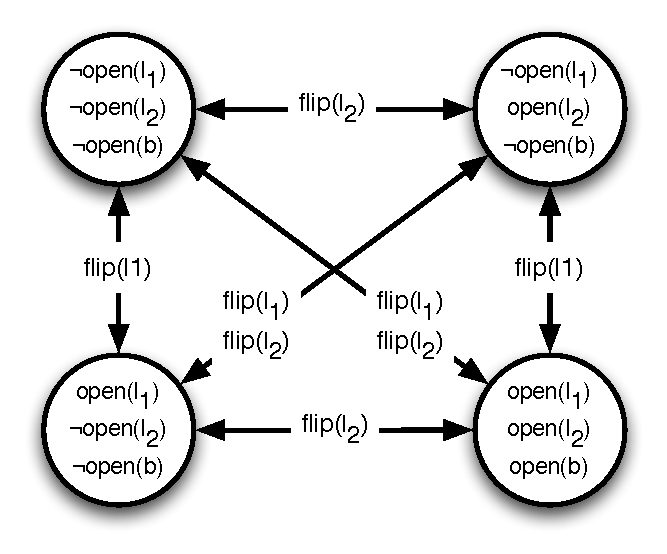
\includegraphics[scale=.5]{../images/briefcase.pdf}
    \caption{Lin's Briefcase Transition Diagram}
    \label{fig:briefcase}
\end{figure}
\lstinputlisting[language=Lisp, caption=Lin's Briefcase Domain Description in PDDL, label=lst:pddl-briefcase]{briefcase-domain.pddl}
\lstinputlisting[language=Lisp, caption=Lin's Briefcase Problem Instance in PDDL, label=lst:pddl-briefcase-problem]{briefcase-problem.pddl}

\subsubsection{Blocks World}
The Blocks World domain is one of the most common benchmark domains in planning as well as in AI; thus, some degree of familiarity with the problem is assumed. We include it in this discussion not only because it is a standard example, but also because it poses an interesting challenge to the planner: the Blocks World may contain some blocks which are irrelevant to the goal state or which are already in the desired configuration in the initial state. 

\lstinputlisting[language=Lisp, caption=Blocks World Domain Description in PDDL, label=lst:pddl-blocks]{blocks-domain.pddl}
\lstinputlisting[language=Lisp, caption=Blocks World Problem Instance in PDDL, label=lst:pddl-blocks-problem]{blocks-problem.pddl}

\subsubsection{Electrical Circuit}
\begin{figure}[htbp]
    \centering
        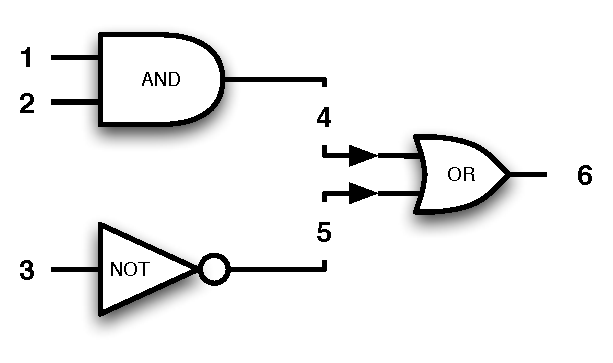
\includegraphics[scale=.5]{../images/circuit.pdf}
    \caption{Electrical Circuit Diagram}
    \label{fig:circuit}
\end{figure}

The simple electrical circuit domain is an interesting domain, because it consists almost entirely of static causation. In order to reify the domain in PDDL such that FF would be able to find plans, we had to introduce additional actions which represent the ``activation'' of a gate; this is the result of the fact that FF does not support derived literals as a result of the evaluation of axioms (see \cite{Thiebaux:2003ys} for a detailed discussion of PDDL axioms). It is possible that the use of a different planner which allowed for this more expressive syntax could result in a decrease in performance, especially with a more complex problem instance. 

\lstinputlisting[language=Lisp, caption=Electrical Circuit Domain Description in PDDL, label=lst:pddl-electrical]{circuit-domain.pddl}
\lstinputlisting[language=Lisp, caption=Electrical Circuit Problem Instance in PDDL, label=lst:pddl-electrical-problem]{circuit-problem.pddl}

\subsubsection{Towers of Hanoi}
The Towers of Hanoi domain is also a common domain across several realms of AI. We included this domain simply to demonstrate the difference between its representation in PDDL and A-Prolog (but not necessarily to highlight a particular shortcoming or advantage of either approach). This is one case where A-Prolog makes use of static causal laws (derived literals), but the PDDL representation does not require additional actions to express the same effects: specifically, determining whether a disc or peg becomes clear. In the PDDL representation, a disc or peg becomes clear as an effect of moving another disc off of the top of it; in the A-Prolog representation, however, a disc or peg becomes clear at some time $t$ if there is no disc on it at that time. 

\lstinputlisting[language=Lisp, caption=Towers of Hanoi Domain Description in PDDL, label=lst:pddl-hanoi]{hanoi-domain.pddl}
\lstinputlisting[language=Lisp, caption=Towers of Hanoi Problem Description in PDDL, label=lst:pddl-hanoi-problem]{hanoi-problem.pddl}